\chapter{Optical lattices and the Bose-Hubbard model}

\NOTE{intro}

\label{sec:chapter_2}

\section{The Bose-Hubbard Model}

We consider a 3D lattice potential with cubic symmetry and spacing $d$:

\begin{equation}
    V(\bm{r})=V_{0}\left[\sin ^{2}\left(\frac{k_{d}}{2} x\right)+\sin ^{2}\left(\frac{k_{d}}{2} y\right)+\sin ^{2}\left(\frac{k_{d}}{2} z\right)\right] + V_{\mathrm{ext}} (x,y,z)
\end{equation}

\noindent where $k_d=\frac{2 \pi}{d}$ is the associated wavevector, $V_0$ the lattice amplitude. For convenience, $V_0$ is usually expressed in units of recoil energy $V_0 = s E_{\rm{r}}$ with $E_r=h^2/ 8 m d^2$. The term $V_{\mathrm{ext}} (x,y,z)$ denotes a harmonic potential related to the Gaussian shape of the lattice beams. For simplicity of calculations, we will only treat here the homogeneous case $V_{\mathrm{ext}} (x,y,z)=0$.

We consider an ensemble of $N$ atoms that interact with one another with the potential $U_{\rm{int}} ( \bm{r}_1, \bm{r}_2)$ loaded in the lattice potential $V(\bm{r})$. The Hamiltonian of the system writes:

\begin{equation}
    \hat{H}=\sum_{i=1}^{N} \frac{\bm{p}_{i}^{2}}{2 m}+\sum_{i=1}^{N} V\left(\bm{r}_{i}\right) + \sum_{i}^{N} \sum_{j>i}^{N} U_{\text{int}}\left(\bm{r}_{i}, \bm{r}_{j}\right)
\end{equation}

\subsubsection{Non-interacting lattice gas}

To begin, we will not consider interactions and study the simplified Hamiltonian:

\begin{equation}
    \hat{H}_0=\sum_{i=1}^{N} \frac{\bm{p}_{i}^{2}}{2 m}+\sum_{i=1}^{N} V\left(\bm{r}_{i}\right)
\end{equation}

\noindent As the Hamiltonian is separable along the 3 directions of space and the gas of atoms is non-interacting, we can simply work with the one-dimensional, single particle Hamiltonian:

\begin{equation}
    \hat{H}_1 = \frac{p_x}{2m} + \sin^2 \Big(\frac{k_d}{2} x \Big)
\end{equation}

\noindent To find the eigenstates of this Hamiltonian, we use the Bloch's theorem \cite{ashcroft1976solid}:

\begin{tcolorbox}[colback=red!5!white,colframe=red!75!black,title=\textbf{Bloch's theorem}]
\label{sec:bloch}
The eigenstates of a Hamiltonian corresponding to a spatially periodic potential $V(\bm{r})$ on a lattice $\mathcal{B}$ are Bloch waves $\psi_{\bm{q}}(\bm{r})$, product of a plane-wave $e^{i \bm{r}.\bm{q}}$ and a periodical function on $\mathcal{B}$, $u_{\bm{q}} (\bm{r})$.
\end{tcolorbox}

We therefore look eigenstates of the form:

\begin{equation}
    \psi_{n,q} (x)= e^{iqx} u_{n,q} (x)
    \label{eq:bloch_wave}
\end{equation}

\noindent with $n \in \N$ and $q$ the \textbf{quasi-impulsion} defined in the interval $[-k_d/2, k_d/2]$ called the \textbf{first Brillouin zone}. In order to determine the functions $u_{\bm{q}} (\bm{r})$, we inject equation \ref{eq:bloch_wave} in the eigenvalue equation to find that they must verify:

\begin{equation}
    \left[\frac{\left(p_{x}+\hbar q\right)^{2}}{2 m}+V_{0} \sin ^{2}\left(\frac{k_{a}}{2} x\right)\right] u_{n, q}(x)=E_{n}(q) u_{n, q}(x)
\end{equation}

The Bloch energy bands $E_{n}(q)$ and the Bloch functions $u_{n, q}(x)$ can be easily numerically calculated. We plot on Fig.-\ref{fig:bloch_bands} the first five energy bands as a function of $q$ in the first Brillouin zone for various values of the lattice amplitude $V_0$. Interestingly, we see that a gap appears between the different bands as we increase $V_0$.

\begin{figure}
    \centering
    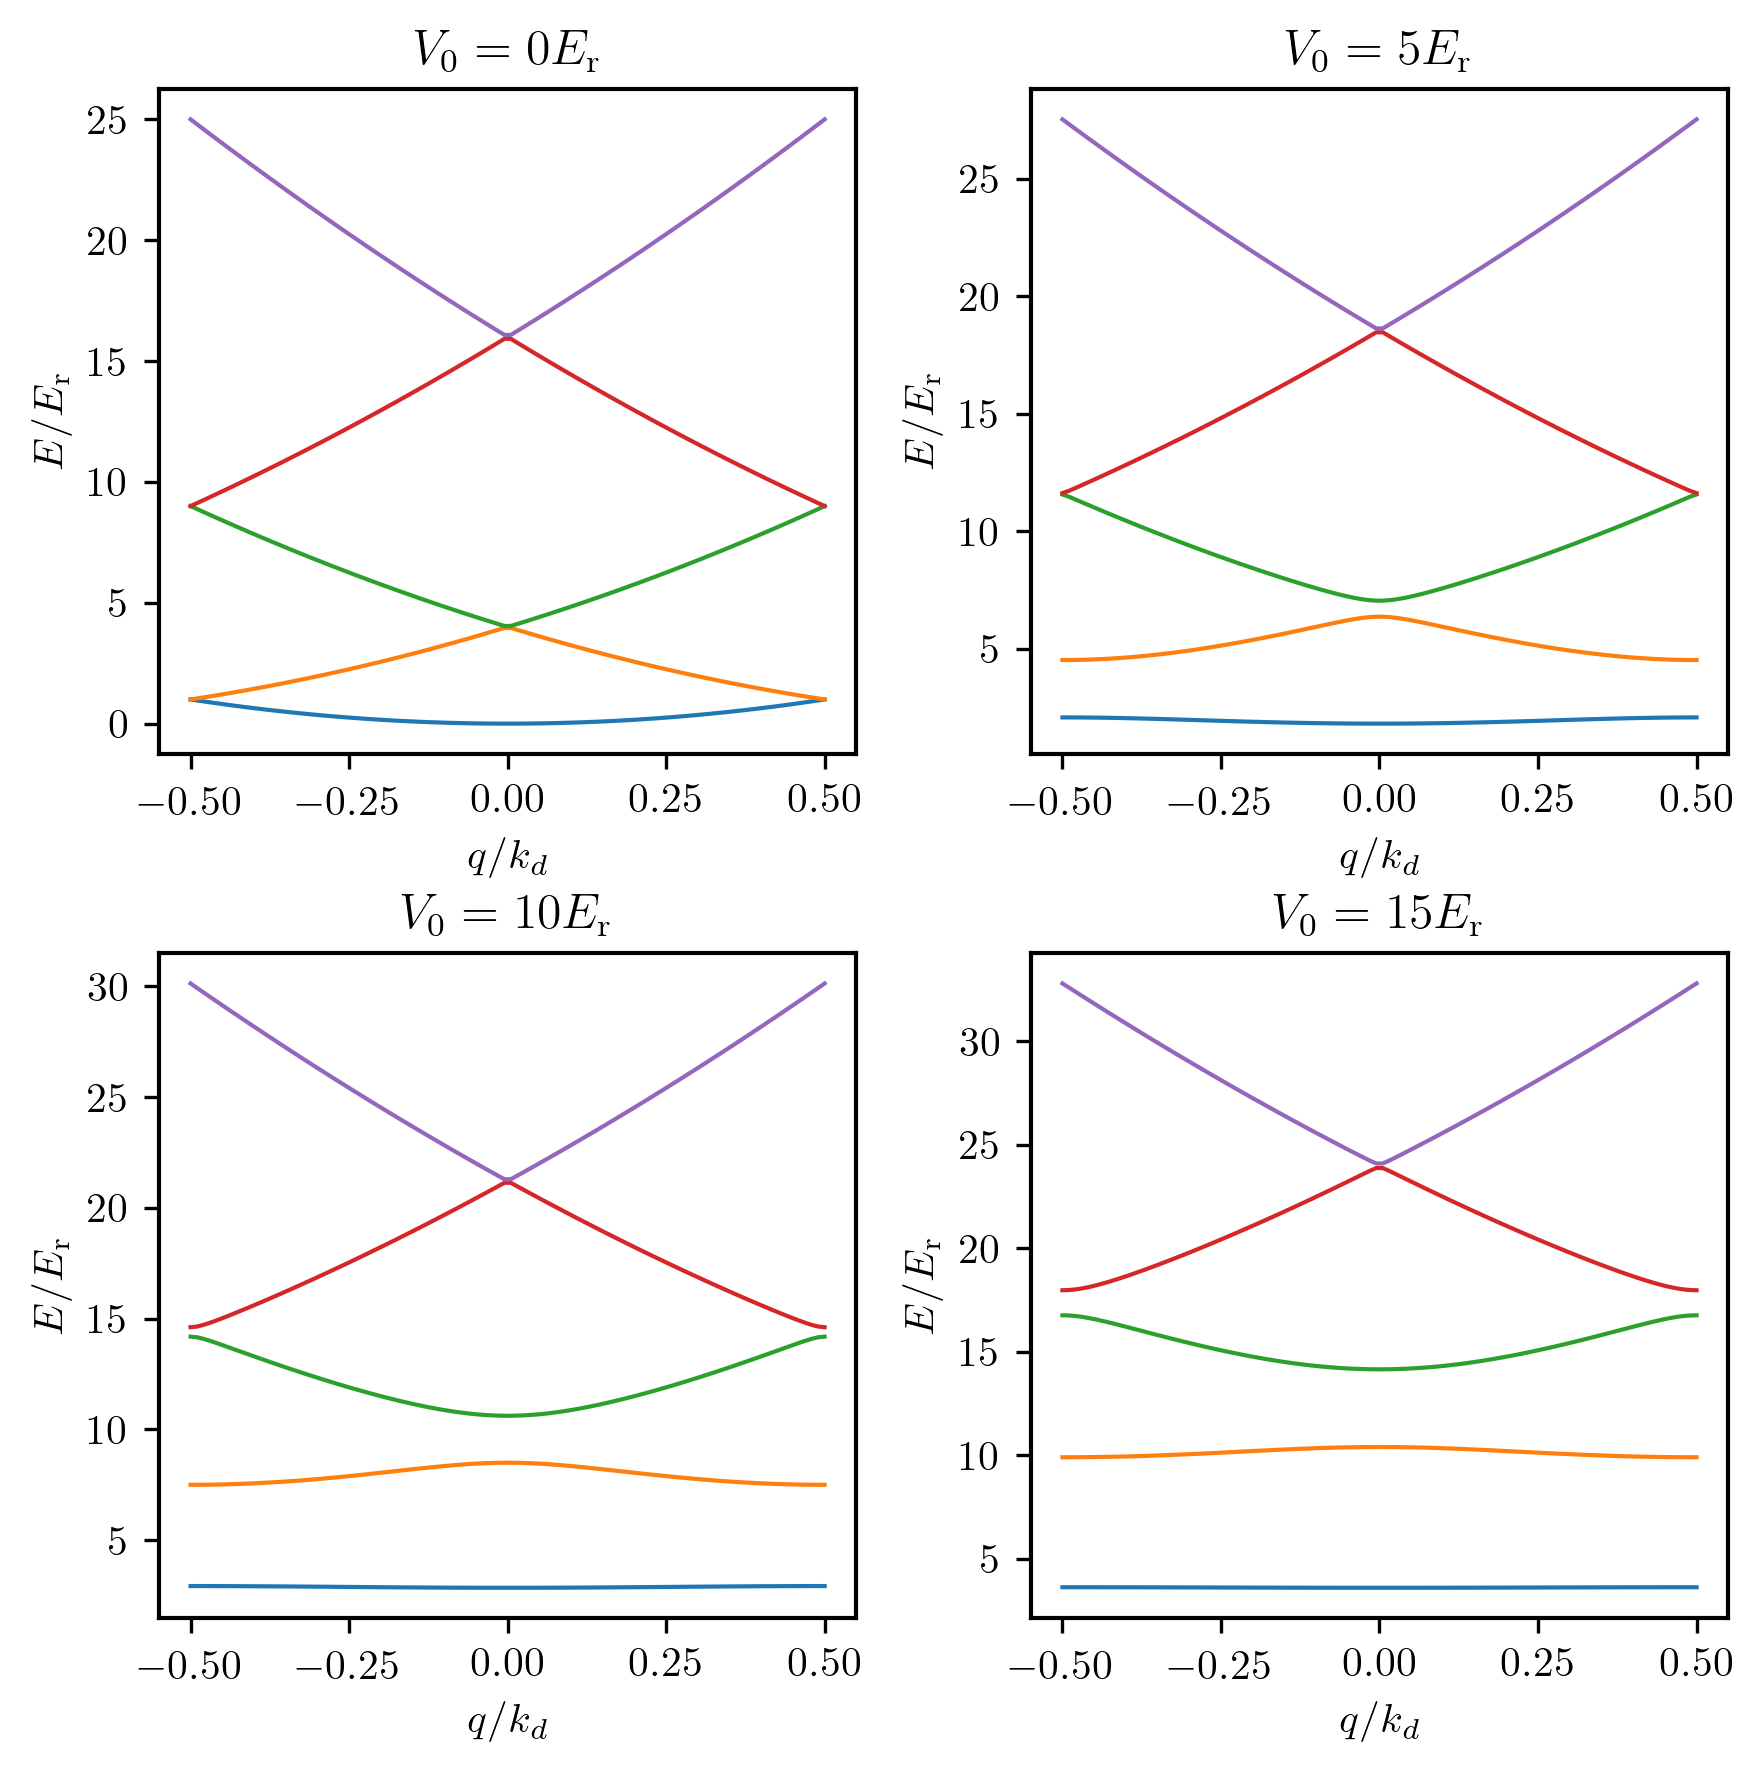
\includegraphics[width=\textwidth]{Fig/Chapter2/bloch_bands.png}
    \caption{First five Bloch energy bands for various lattice amplitudes $V_0$. The gap between the first bands increases as $V_0$ increases.}
    \label{fig:bloch_bands}
\end{figure}


\section{The Mott transition}

\section{Accessing the in-trap momentum distribution}

\subsection{The far-field regime}

\subsection{Mean-field interactions}

\subsection{Beyond mean-field interactions}

